% Provenance (never printed): see sources/outline_sources.md (Year 3:
% geomorphology, hillslope processes, river incision, landscape evolution).
% Brief: sources/book5/BRIEFS.md, ch. 18. Curves from
% figdata/bachelor-3/hillslope.py, stream_profile.py and varden_river.py.
% Exercise and problem values in the Book 5 scratch calculator calc/ch18.py.
% The upland west of the Varden Hills, its river, its tributaries, its
% uplift rate and its base-level fall are invented; the outlet elevation is
% the region model's river at the west edge of the map.
\chapter{Geomorfologi Kuantitatif}\label{ch:b3:quantitative-geomorphology}

Sungai yang melintasi pegunungan yang terangkat memiliki undakan pada profil memanjangnya: air terjun,
dengan ngarai di bawahnya dan lembah yang lebih landai di atasnya. Undakan itu tidak tetap
di tempat ia terbentuk. Undakan itu bergerak ke hulu, beberapa milimeter atau beberapa meter
per tahun, dan posisinya adalah jam yang mulai berjalan ketika dasar sungai
diturunkan. Membaca jam itu, dan laju yang tertulis dalam bentuk bukit
dan sungai, memerlukan dua hukum kekekalan dan dua hukum transpor: satu untuk
tanah yang merayap menuruni lereng, satu untuk batuan dasar yang dipotong sungai.

\begin{recall}
Pelapukan, erosi, pengendapan, bentuk lahan, dan keseimbangan antara pengangkatan
dan erosi dibahas dalam volume-volume sekolah, begitu pula pantulan isostatik dan lembah
glasial berbentuk U. Laju denudasi, tegangan geser dasar, dan parameter Shields
dibahas dalam volume Tahun 1, pada bab tentang erosi dan transpor;
model elevasi digital pada bab tentang peta geologi; isostasi Airy
dibahas pada bab tentang isostasi dan anomali gravitasi. \omterm{def:b3:advanced-geochronology:cosmogenic}{Nuklida kosmogenik}
dan laju erosi yang diturunkan darinya dibahas pada
Bab~\ref{ch:b3:advanced-geochronology}, \omterm{def:b3:orogenic-wedges:thermochronology}{termokronologi} dan
\omterm{def:b3:orogenic-wedges:age-elevation}{hubungan umur--elevasi} dibahas pada Bab~\ref{ch:b3:orogenic-wedges}. Persamaan
difusi ada dalam buku fisika.
\end{recall}

\section{Lereng-lereng}\label{sec:b3:quantitative-geomorphology:hillslopes}

Pada bukit yang tertutup tanah, tanah bergerak menuruni lereng butir demi butir: hewan penggali
melemparkannya, akar mengangkatnya, pembekuan dan pembasahan memekarkannya, dan setiap
gangguan memungkinkan gravitasi menggesernya sedikit. Dirata-ratakan selama berabad-abad, fluks
tanah sebanding dengan lerengnya.

\begin{definition}[Difusi lereng]\label{def:b3:quantitative-geomorphology:diffusion}
Yang disebut \emph{difusi lereng}\index{difusi lereng} adalah pengangkutan tanah yang lambat
menuruni lereng yang fluks volumenya per satuan lebar lereng,
$\vec q$, sebanding dengan gradien elevasi permukaan $z$:
$\vec q = -\kappa\,\nabla z$. Koefisien $\kappa$, dalam
\unit{m^2/yr}, adalah difusivitas lereng.
\end{definition}

\begin{theorem}[Difusi pada lereng]\label{thm:b3:quantitative-geomorphology:diffusion}
Misalkan batuan terangkat dengan laju $U$ relatif terhadap alur yang membatasi
sebuah lereng, tanah dan batuan memiliki massa jenis yang sama, dan tanah bergerak melalui
\omterm{def:b3:quantitative-geomorphology:diffusion}{difusi lereng} dengan $\kappa$ seragam. Maka elevasi permukaan memenuhi
\[
\frac{\partial z}{\partial t} = U + \kappa\,\nabla^2 z ,
\]
yaitu persamaan difusi dengan suku sumber.
\end{theorem}

\begin{proof}
Ambil luasan kecil $\delta S$ dari lereng. Volumenya berubah karena pengangkatan,
$U\,\delta S$ per satuan waktu, dan karena tanah yang mengalir keluar melalui
tepinya, $\oint \vec q\cdot\vec n\,\mathrm{d}\ell = (\nabla\cdot\vec q)\,\delta S$.
Dengan demikian $\partial z/\partial t = U - \nabla\cdot\vec q$; dengan $\vec q = -\kappa
\nabla z$ dan $\kappa$ seragam, $\nabla\cdot\vec q = -\kappa\nabla^2 z$.
\end{proof}

Sebuah sesar atau garis pantai memotong tebing terjal dalam satu waktu; sesudahnya tebing itu hanya
berdifusi. Mulai dari undakan vertikal dengan setengah tinggi $a$ pada lereng medan jauh
$b$, solusi dalam satu dimensi adalah
\[
z(x,t) = a\,\operatorname{erf}\!\left(\frac{x}{2\sqrt{\kappa t}}\right) + b\,x ,
\qquad
\left.\frac{\partial z}{\partial x}\right|_{x=0} = \frac{a}{\sqrt{\pi\kappa t}} + b .
\]
Bentuknya hanya bergantung pada hasil kali $\kappa t$: profil terukur memberikan
$\kappa t$, dan umur independen memberikan $\kappa$, atau $\kappa$ yang diketahui
memberikan umur, yakni \emph{umur morfologis}. Tebing terjal di wilayah semi-arid
dengan tanah berbutir dan vegetasi jarang memberikan $\kappa$ antara
$10^{-3}$ dan \qty{e-2}{m^2/yr}; pegunungan pesisir yang lembap dan bervegetasi rapat
sekitar \qty{5e-3}{m^2/yr}.
% ledger: whipple04:scarp-erf, whipple04:scarp-kappa

\begin{omfigure}
\begin{tikzpicture}
\begin{groupplot}[group style={group size=2 by 1, horizontal sep=1.6cm},
  width=0.48\linewidth, height=0.36\linewidth, tick label style={font=\scriptsize},
  label style={font=\small}, legend style={font=\scriptsize, draw=none, fill=none}]
\nextgroupplot[xlabel={jarak $x$ (m)}, ylabel={$z$ (m)}, xmin=-40, xmax=40,
  ymin=-5, ymax=5, legend pos=north west]
% computed in figdata/bachelor-3/hillslope.py
\addplot[black!50, densely dashed] table[x=x, y=z0] {figdata/out/bachelor-3-hillslope-scarp.dat};
\addplot[omDef, thick] table[x=x, y=z1] {figdata/out/bachelor-3-hillslope-scarp.dat};
\addplot[omProp, thick] table[x=x, y=z2] {figdata/out/bachelor-3-hillslope-scarp.dat};
\addplot[omThm, thick] table[x=x, y=z3] {figdata/out/bachelor-3-hillslope-scarp.dat};
\legend{awal, \qty{2}{ka}, \qty{10}{ka}, \qty{40}{ka}}
\nextgroupplot[xlabel={jarak dari pembagi aliran (m)}, ylabel={tinggi (m)},
  xmin=-150, xmax=150, ymin=0, ymax=200, xtick={-150,-75,0,75,150}]
\addplot[omMeth, thick] table[x=x, y=z1] {figdata/out/bachelor-3-hillslope-hill.dat};
\addplot[omDef, thick] table[x=x, y=z2] {figdata/out/bachelor-3-hillslope-hill.dat};
\addplot[omThm, thick] table[x=x, y=z3] {figdata/out/bachelor-3-hillslope-hill.dat};
\node[font=\scriptsize, anchor=north] at (axis cs:0,45) {0.0215};
\node[font=\scriptsize, anchor=north] at (axis cs:0,94) {0.043};
\node[font=\scriptsize, anchor=north] at (axis cs:0,184) {\qty{0.086}{mm/yr}};
\end{groupplot}
\end{tikzpicture}

\par\smallskip{\small Kiri, tebing terjal dengan pergeseran \qty{5}{m} pada lereng sebesar
0.05, berdifusi dengan $\kappa = \qty{5e-3}{m^2/yr}$: langkah awal
(putus-putus) dan profil setelah 2, 10 dan \qty{40}{ka}. Kanan, bukit tunak
dengan setengah lebar \qty{150}{m} dan $\kappa$ yang sama (tinggi di atas
alur), menurun dengan laju
0.0215, 0.043 dan \qty{0.086}{mm/yr}: parabola yang reliefnya serta kelengkungan
puncaknya sebanding dengan laju erosi.}\label{fig:b3:quantitative-geomorphology:hillslope}
\end{omfigure}
% ledger: whipple04:scarp-kappa

Ketika sebuah bukit telah terangkat dan tererosi cukup lama, bentuknya berhenti
berubah: setiap titik turun dengan laju batuan terangkat.

\begin{proposition}[Kelengkungan puncak mengukur laju erosi]\label{prop:b3:quantitative-geomorphology:curvature}
Pada lereng bukit dalam \omterm{def:b3:quantitative-geomorphology:steady-profile}{keadaan tunak} di bawah \omterm{def:b3:quantitative-geomorphology:diffusion}{difusi lereng}, laju erosi
$E$, yang sama dengan $U$, adalah
\[
E = -\kappa\,\nabla^2 z .
\]
Dalam satu dimensi, profilnya berupa parabola $z = z_0 - E x^2/(2\kappa)$,
dengan relief $E L^2/(2\kappa)$ antara punggungan pemisah dan alur yang berjarak
$L$ dari titik itu.
\end{proposition}

\begin{proof}
Dengan menetapkan $\partial z/\partial t = 0$ pada teorema, diperoleh $\kappa\nabla^2 z =
-U = -E$. Dalam satu dimensi, dua kali integrasi dengan $\mathrm{d}z/\mathrm{d}x =
0$ di punggungan pemisah menghasilkan parabola, dan nilainya di $x = L$ memberikan relief.
\end{proof}

Kelengkungan, besaran geometris yang diukur pada model elevasi digital, dengan demikian
dapat dibaca sebagai laju begitu $\kappa$ diketahui: makin curam dan makin tajam
membulat puncak bukitnya, makin cepat pula bentang alam itu tererosi. Tanah sendiri terbentuk dari
batuan di bawahnya dengan laju yang bergantung pada seberapa banyak tanah yang sudah menutupinya.

\begin{definition}[Fungsi produksi tanah]\label{def:b3:quantitative-geomorphology:soil-production}
Yang disebut \emph{fungsi produksi tanah}\index{fungsi produksi tanah} memberikan
laju $P$ batuan dasar berubah menjadi tanah sebagai fungsi
ketebalan tanah $h$; umumnya diambil sebagai $P = P_0\,e^{-h/h_0}$, dengan
$P_0$ adalah laju pada batuan telanjang dan $h_0$ panjang berorde pecahan meter.
\end{definition}

Dalam \omterm{def:b3:quantitative-geomorphology:steady-profile}{keadaan tunak}, bidang batas tanah-batuan turun dengan laju
permukaan, $P(h) = E$, sehingga ketebalan tanah $h = h_0 \ln(P_0/E)$: erosi yang lebih cepat
berarti tanah lebih tipis, dan di tempat $E$ melampaui $P_0$ tanah
terkikis dan batuan telanjang, dibatasi oleh pelapukan, tersingkap. \omterm{def:b3:advanced-geochronology:cosmogenic}{Laju
produksi} tanah tercepat yang terukur berorde \qty{0.5}{mm/yr}.
% ledger: whipple04:soil

Difusi linear gagal pada lereng curam. Ketika gradien mendekati sebuah
ambang, butir-butir menggelinding dan meluncur dalam hentakan, dan tanah longsor dangkal mengupas
lapisan tanahnya.

\begin{definition}[Gradien lereng kritis]\label{def:b3:quantitative-geomorphology:critical}
Yang disebut \emph{gradien lereng kritis}\index{gradien lereng kritis}
$S_c$ adalah gradien tempat fluks tanah tumbuh tanpa batas; dalam
hukum transpor nonlinear yang banyak dipakai, $q = \kappa S/[1 - (S/S_c)^2]$.
\end{definition}

Lereng yang jauh lebih landai daripada $S_c$ berperilaku seperti difusi linear; lereng yang
tererosi cepat menjadi makin curam menuju $S_c$ dan berbentuk planar, gradiennya ditentukan oleh
ambang, bukan oleh laju erosi.
% ledger: whipple04:nonlinear

\begin{inthefield}[Memindai lereng bukit]
Sebuah tim yang menyurvei punggungan berselimut tanah memasang pemindai laser terestrial pada
tripod beberapa puluh meter dari punggungan. Setiap pemindaian merekam jutaan
titik, jarak dan arah ke permukaan tanah, melalui celah-celah di
antara rumput dan semak; titik-titik dari beberapa stasiun pemindai digabungkan
menjadi satu awan, diregistrasi ke target yang disurvei dengan penerima satelit,
dan pantulan terakhir disimpan untuk menghilangkan vegetasi. Awan titik tanah telanjang
dipetakan ke dalam kisi menjadi model elevasi dengan sel berukuran desimeter, dihaluskan sepanjang beberapa
meter, dan Laplacian-nya dihitung di punggungan. Tim kemudian membandingkan
kelengkungan puncak punggungan yang tererosi dengan laju yang diukur dengan
\omterm{def:b3:advanced-geochronology:cosmogenic}{nuklida kosmogenik}: jika diplot satu sama lain, keduanya memberikan difusivitas
lereng sebagai kemiringan garis, seperti yang diprediksi proposisi.
\end{inthefield}

\section{Penorehan sungai}\label{sec:b3:quantitative-geomorphology:rivers}

Di tempat sungai mengalir di atas batuan dasar, ia menggerus ke bawah dengan mencabut blok-blok,
dengan abrasi di bawah muatan dasarnya, dan dengan kavitasi. Semuanya sebanding dengan tegangan
geser yang dikerjakan aliran pada dasarnya, atau daya yang dihabiskan di sana, dan keduanya
bertambah seiring debit dan kemiringan. Debit bertambah seiring luas daerah tangkapan, sehingga luas
mewakili debit.

\begin{definition}[Hukum daya sungai]\label{def:b3:quantitative-geomorphology:stream-power}
Yang disebut \emph{hukum daya sungai}\index{hukum daya sungai} memberikan laju
penorehan vertikal $E$ sungai batuan dasar sebagai
\[
E = K A^m S^n ,
\]
dengan $A$ adalah luas daerah tangkapan di hulu titik itu, $S$ gradien alur,
$m$ dan $n$ eksponen positif, dan $K$ koefisien erodibilitas
yang merangkum kekuatan batuan, iklim, dan lebar alur.
\end{definition}

Untuk proses yang sebanding dengan tegangan geser atau dengan daya aliran satuan,
$m/n$ mendekati 0.5. Survei alur badland yang terbentuk pada batuan lemah selama
sekitar 20 tahun menemukan laju penorehan sebanding dengan $A^{0.44}S^{0.68}$.
% ledger: whipple04:spim

\begin{definition}[Penorehan terbatas-pelepasan dan terbatas-angkutan]\label{def:b3:quantitative-geomorphology:limited}
Penorehan bersifat \emph{terbatas-pelepasan}\index{penorehan terbatas-pelepasan} ketika sungai
dapat membawa pergi lebih banyak sedimen daripada yang diterimanya, sehingga laju penurunan
dasarnya ditentukan oleh seberapa cepat ia melepaskan batuan dari dasar: \omterm{def:b3:quantitative-geomorphology:stream-power}{hukum daya sungai} berlaku.
Penorehan itu
bersifat \emph{terbatas-angkutan}\index{penorehan terbatas-angkutan} ketika sungai
membawa semua sedimen yang dapat dibawanya, sehingga dasarnya hanya diturunkan di tempat
kapasitas angkut bertambah ke hilir, dengan laju yang ditentukan oleh divergensi
fluks sedimen.
\end{definition}

Sungai \omterm{def:b3:quantitative-geomorphology:limited}{terbatas-angkutan} berperilaku mirip lereng bukit: fluks bergantung
pada kemiringan, dan profilnya berkembang dengan persamaan seperti difusi yang membulatkan
setiap undakan. Sungai \omterm{def:b3:quantitative-geomorphology:limited}{terbatas-pelepasan} menjaga undakan tetap tajam dan memindahkannya,
seperti ditunjukkan subbagian berikutnya. Sungai pegunungan dengan lantai batuan dasar dan
kerikil tipis biasanya lebih dekat ke yang pertama; sungai di atas aluvium tebal ke yang
kedua.

\begin{omfigure}
\begin{tikzpicture}[x=0.55cm, y=0.55cm, font=\scriptsize,
  declare function={f(\x)=2.1+3.5*(1-(\x-0.5)/10)^2;
    tl(\x,\l)=f(\x)-1.1*exp(-(10.5-\x)/\l);}]
\begin{scope}
\draw[->] (0,0) -- (11.5,0) node[below left] {jarak ke hilir};
\draw[->] (0,0) -- (0,6) node[above right] {$z$};
\draw[black!50, densely dashed] plot[domain=0.5:10.5, samples=40] (\x,{f(\x)});
\draw[omDef, thick] plot[domain=0.5:6.5, samples=30] (\x,{f(\x)}) -- plot[domain=6.5:10.5, samples=20] (\x,{f(\x)-1.1});
\draw[omThm, thick] plot[domain=0.5:3.5, samples=20] (\x,{f(\x)}) -- plot[domain=3.5:10.5, samples=30] (\x,{f(\x)-1.1});
\draw[->, black!70] (6.3,4.1) -- (3.8,4.75);
\node[anchor=west, align=left] at (5.6,5.3) {terbatas-pelepasan:\\ undakan bergerak ke hulu};
\node at (5.5,-0.7) {(a)};
\end{scope}
\begin{scope}[xshift=7.2cm]
\draw[->] (0,0) -- (11.5,0) node[below left] {jarak ke hilir};
\draw[->] (0,0) -- (0,6) node[above right] {$z$};
\draw[black!50, densely dashed] plot[domain=0.5:10.5, samples=40] (\x,{f(\x)});
\draw[omDef, thick] plot[domain=0.5:10.5, samples=40] (\x,{tl(\x,1.2)});
\draw[omThm, thick] plot[domain=0.5:10.5, samples=40] (\x,{tl(\x,3.5)});
\node[anchor=west, align=left] at (5.0,5.3) {terbatas-angkutan:\\ penurunan berdifusi ke hulu};
\node at (5.5,-0.7) {(b)};
\end{scope}
\end{tikzpicture}

\par\smallskip{\small Respons sungai terhadap penurunan \omterm{def:b3:quantitative-geomorphology:knickpoint}{dasar erosinya}
(putus-putus: profil sebelum penurunan; biru, lalu merah: dua waktu berikutnya),
skematik. (a) Sungai \omterm{def:b3:quantitative-geomorphology:limited}{terbatas-pelepasan} mempertahankan \omterm{def:b3:quantitative-geomorphology:knickpoint}{titik tekuk} tajam yang
bergerak ke hulu; di bawahnya profil tetap berbentuk lama, hanya turun. (b) Sungai
\omterm{def:b3:quantitative-geomorphology:limited}{terbatas-angkutan} menurunkan seluruh profilnya secara bertahap, paling banyak dekat
muara.}\label{fig:b3:quantitative-geomorphology:regimes}
\end{omfigure}

Jika batuan naik dengan laju seragam $U$ terhadap muara sungai, dan $K$,
$m$, $n$ seragam, sungai berkembang sebagai $\partial z/\partial t = U - K A^m
S^n$.

\begin{definition}[Profil sungai keadaan tunak]\label{def:b3:quantitative-geomorphology:steady-profile}
Profil sungai berada dalam \emph{keadaan tunak}\index{profil sungai keadaan tunak}
ketika ketinggiannya tidak lagi berubah terhadap waktu: di setiap titik, penggerusan
menyeimbangkan pengangkatan batuan terhadap muara.
\end{definition}

\begin{theorem}[Profil keadaan tunak di bawah hukum daya sungai]\label{thm:b3:quantitative-geomorphology:steady}
Jika $U$, $K$, $m$, dan $n$ seragam, sungai \omterm{def:b3:quantitative-geomorphology:limited}{terbatas-pelepasan} dalam
\omterm{def:b3:quantitative-geomorphology:steady-profile}{keadaan tunak} memiliki gradien
\[
S = \left(\frac{U}{K}\right)^{1/n} A^{-m/n} .
\]
\end{theorem}

\begin{proof}
Pada \omterm{def:b3:quantitative-geomorphology:steady-profile}{keadaan tunak} $\partial z/\partial t = 0$, sehingga $K A^m S^n = U$, maka $S^n
= (U/K)A^{-m}$; dengan mengambil akar ke-$n$ diperoleh hasilnya.
\end{proof}

\begin{omfigure}
\begin{tikzpicture}
\begin{groupplot}[group style={group size=2 by 1, horizontal sep=1.7cm},
  width=0.48\linewidth, height=0.33\linewidth, tick label style={font=\scriptsize},
  label style={font=\small}]
\nextgroupplot[xlabel={jarak dari pemisah air (km)}, ylabel={$z$ (m)},
  xmin=0, xmax=12, ymin=150, ymax=420]
% computed in figdata/bachelor-3/stream_profile.py
\addplot[omDef, thick] table[x=d, y=z] {figdata/out/bachelor-3-stream_profile-steady.dat};
\nextgroupplot[xmode=log, ymode=log, xlabel={luas daerah aliran $A$ (\unit{km^2})},
  ylabel={gradien $S$}, xmin=0.1, xmax=100, ymin=0.003, ymax=0.2]
\addplot[omDef, thick] table[x=A, y=S] {figdata/out/bachelor-3-stream_profile-steady.dat};
\addplot[only marks, mark=*, mark size=1.4pt, omThm] table[x=A, y=S] {figdata/out/bachelor-3-stream_profile-sa.dat};
\addplot[omThm, densely dashed] table[x=A, y=S] {figdata/out/bachelor-3-stream_profile-fit.dat};
\end{groupplot}
\end{tikzpicture}

\par\smallskip{\small Profil \omterm{def:b3:quantitative-geomorphology:steady-profile}{keadaan tunak} sungai dataran tinggi rekaan
di sebelah barat Varden Hills ($U = \qty{0.043}{mm/yr}$, $K =
\qty{e-6}{yr^{-1}}$, $m = 0.5$, $n = 1$), dari hulu alurnya ke
muara pada \qty{170}{m}. Kanan, gradien terhadap luas: model (biru
garis) dan dua belas gradien yang diukur pada segmen sepanjang \qty{200}{m} dengan
sebaran sekitar \qty{10}{\percent} (titik merah), garis kuadrat terkecilnya
(putus-putus) memiliki kemiringan $-0.47$.}\label{fig:b3:quantitative-geomorphology:profile}
\end{omfigure}

Gradien turun sebagai pangkat luas: profil itu cekung ke atas. Sungai
sebenarnya mengikuti hukum pangkat semacam itu meskipun asumsi teorema
diragukan, sehingga dua angka merangkum sebuah profil.
% ledger: whipple04:steepness

\begin{definition}[Indeks kecuraman alur dan kecekungan]\label{def:b3:quantitative-geomorphology:indices}
Jika gradien sungai mengikuti $S = k_s A^{-\theta}$, eksponen
$\theta$ disebut \emph{indeks kecekungan}\index{indeks kecekungan} dan
koefisien $k_s$ disebut \emph{indeks kecuraman alur}\index{indeks kecuraman alur}.
Untuk membandingkan sungai, $\theta$ ditetapkan pada nilai acuan bersama
$\theta_{\mathrm{ref}}$, dan $k_{sn} = S A^{\theta_{\mathrm{ref}}}$ adalah
kecuraman ternormalisasi.
\end{definition}

Menurut teorema, $\theta = m/n$ dan $k_s = (U/K)^{1/n}$: pada
erodibilitas tertentu, sungai lebih curam di tempat batuan naik lebih cepat. Peta kecuraman
suatu pegunungan karena itu memperlihatkan pengangkatannya.


Gradien adalah turunan ketinggian yang berderau dan sebarannya lebar. Mengintegrasikan
profil justru memakai ketinggian, yang lebih baik diukur.

\begin{definition}[Analisis chi]\label{def:b3:quantitative-geomorphology:chi}
Yang disebut \emph{analisis chi}\index{analisis chi} memplot ketinggian titik-titik
pada jaringan sungai terhadap koordinat
\[
\chi(x) = \int_{x_b}^{x} \left(\frac{A_0}{A(x')}\right)^{\theta}
\mathrm{d}x' ,
\]
dengan $x$ adalah jarak sepanjang alur ke hulu dari titik dasar
$x_b$, $A_0$ luas acuan, dan $\theta$ \omterm{def:b3:quantitative-geomorphology:indices}{indeks kecekungan}; $\chi$ memiliki
dimensi panjang.
\end{definition}

\begin{proposition}[Transformasi chi meluruskan profil keadaan tunak]\label{prop:b3:quantitative-geomorphology:chi}
Di bawah asumsi teorema \omterm{def:b3:quantitative-geomorphology:steady-profile}{keadaan tunak}, dengan $\theta = m/n$,
setiap alur dari suatu jaringan yang mengalir ke elevasi dasar $z_b$ memenuhi
\[
z = z_b + \left(\frac{U}{K A_0^{m}}\right)^{1/n} \chi :
\]
semua alur terletak pada satu garis lurus dengan kemiringan $k_s A_0^{-\theta}$ pada
bidang $(\chi, z)$.
\end{proposition}

\begin{proof}
Sepanjang suatu alur, $\mathrm{d}z/\mathrm{d}x = S = k_s A^{-\theta} = k_s
A_0^{-\theta}(A_0/A)^{\theta}$. Mengintegralkan dari $x_b$, tempat $z = z_b$,
menghasilkan $z = z_b + k_s A_0^{-\theta}\chi$, dan $k_s A_0^{-\theta} =
(U/K)^{1/n} A_0^{-m/n}$. Anak sungai bergabung dengan sungai utama di titik pertemuan yang
$z$ dan $\chi$-nya sama dengan sungai utama, dan hubungan yang sama berlaku di hulunya.
\end{proof}

Alur yang menyimpang dari garis tersebut tidak berada dalam \omterm{def:b3:quantitative-geomorphology:steady-profile}{keadaan tunak}, atau melintasi
batuan dengan erodibilitas berbeda, atau telah kehilangan atau menangkap luas daerah aliran: sebuah
anak sungai yang titiknya berada di atas tetangganya pada $\chi$ yang sama sedang
kehilangan luas, sedangkan yang berada di bawah sedang bertumbuh.

\section{Bentang alam transien}\label{sec:b3:quantitative-geomorphology:transient}

\begin{definition}[Dasar erosi dan titik tekuk]\label{def:b3:quantitative-geomorphology:knickpoint}
Yang disebut \emph{dasar erosi}\index{dasar erosi} sebuah sungai adalah elevasi muaranya,
di bawah tingkat itu sungai tidak dapat mengikis: laut, danau, atau sungai utama tempat ia
bergabung. Yang disebut \emph{titik tekuk}\index{titik tekuk} ialah lokasi ketika gradien
profil memanjang sungai meningkat mendadak, dari ruas yang menjadi curam
menuju air terjun.
\end{definition}

\omterm{def:b3:quantitative-geomorphology:knickpoint}{Titik tekuk} dapat bersifat tetap, yaitu saat sungai melintasi lapisan yang lebih keras atau
tebing sesar yang masih aktif, atau dapat bersifat bergerak, yaitu ketika titik itu menjadi kepala dari
respons sungai terhadap perubahan di bawahnya: turunnya \omterm{def:b3:quantitative-geomorphology:knickpoint}{dasar erosi}, atau
pengangkatan yang lebih cepat.
% ledger: whipple04:response

\begin{theorem}[Titik tekuk sebagai gelombang kinematik]\label{thm:b3:quantitative-geomorphology:kinematic}
Misalkan $n = 1$, dengan $U$, $K$, dan $m$ seragam, dan $x$ menyatakan jarak
ke hulu dari muara. Maka $z$ memenuhi
\[
\frac{\partial z}{\partial t} + K A^m \frac{\partial z}{\partial x} = U ,
\]
dan setiap fitur profil, termasuk undakan, merambat ke hulu dengan
kecepatan rambat $c = K A^m$ sambil mempertahankan tingginya. \omterm{def:b3:quantitative-geomorphology:knickpoint}{Titik tekuk} yang
berawal di muara pada $t = 0$ mencapai titik $x$ pada waktu
\[
t(x) = \int_0^x \frac{\mathrm{d}x'}{K A(x')^m} = \frac{\chi(x)}{K A_0^m},
\]
dengan $\chi$ dihitung menggunakan $\theta = m$. Semua \omterm{def:b3:quantitative-geomorphology:knickpoint}{titik tekuk} yang terbentuk dalam suatu jaringan
pada saat yang sama, oleh karena itu, berada pada $\chi$ yang sama, dan pada kontur yang sama.
\end{theorem}

\begin{proof}
Dengan $x$ diukur ke hulu, gradiennya adalah $S = \partial z/\partial x$, dan
persamaan evolusi $\partial z/\partial t = U - K A^m S$ ialah persamaan
yang sudah ditulis. Sepanjang kurva $\mathrm{d}x/\mathrm{d}t = K A(x)^m$, ruas kirinya
adalah turunan total $\mathrm{d}z/\mathrm{d}t$, sehingga $z$ bertambah sebesar $U$ per
satuan waktu sepanjang setiap kurva semacam itu. Dua titik di kedua sisi undakan,
yang terbawa sepanjang kurva bertetangga, memperoleh tinggi yang sama, sehingga undakan
mempertahankan tingginya dan bergerak bersama kurva-kurva itu. Waktu untuk mencapai $x$ adalah
$\int \mathrm{d}x'/c$, yaitu $\chi(x)/(K A_0^m)$ menurut definisi
$\chi$ dengan $\theta = m$. Dalam jaringan, $\chi$ diukur sepanjang setiap
lintasan aliran dari muara yang sama, sehingga waktu yang sama berarti $\chi$ yang sama, dan menurut
proposisi tentang $\chi$, ruas-ruas di bawah \omterm{def:b3:quantitative-geomorphology:knickpoint}{titik tekuk} yang sudah
menyesuaikan diri dengan \omterm{def:b3:quantitative-geomorphology:knickpoint}{dasar erosi} yang baru, membuat semuanya berada pada elevasi yang sama.
\end{proof}

Kecepatan rambat meningkat seiring luas daerah aliran: \omterm{def:b3:quantitative-geomorphology:knickpoint}{titik tekuk} merambat cepat melalui
sungai utama dan melambat di bagian hulu. Waktu yang diperlukan untuk melintasi seluruh
jaringan hingga ke kepala alur adalah \emph{waktu respons} bentang alam,
berorde satu juta tahun untuk laju pengangkatan yang lazim. Bila $n \ne 1$
kecepatan rambat juga bergantung pada kemiringan, dan undakan berubah bentuk: untuk $n >
1$ sisi curamnya mendahului ruas-ruas di sekitarnya dan tetap tajam, sedangkan untuk $n <
1$ undakan itu tertinggal dan menyebar.

\begin{omfigure}
\begin{tikzpicture}
\begin{groupplot}[group style={group size=2 by 1, horizontal sep=1.5cm},
  width=0.5\linewidth, height=0.42\linewidth, tick label style={font=\scriptsize},
  label style={font=\small}, legend style={font=\scriptsize, draw=none, fill=none}]
\nextgroupplot[xlabel={jarak dari pembagi air (km)}, ylabel={$z$ (m)}, xmin=0, xmax=12.2,
  ymin=160, ymax=440, legend pos=north east]
% computed in figdata/bachelor-3/stream_profile.py
\addplot[black!50, densely dashed] table[x=d, y=z0] {figdata/out/bachelor-3-stream_profile-knick.dat};
\addplot[omMeth, thick] table[x=d, y=z1] {figdata/out/bachelor-3-stream_profile-knick.dat};
\addplot[omDef, thick] table[x=d, y=z2] {figdata/out/bachelor-3-stream_profile-knick.dat};
\addplot[omThm, thick] table[x=d, y=z3] {figdata/out/bachelor-3-stream_profile-knick.dat};
\legend{sebelum, \qty{300}{ka}, \qty{600}{ka}, \qty{900}{ka}}
\nextgroupplot[xlabel={$\chi$ (m)}, ylabel={$z$ (m)}, xmin=0, xmax=7500, ymin=160, ymax=520,
  scaled x ticks=false, xtick={0,2000,4000,6000}, xticklabels={0,2000,4000,6000},
  legend pos=north west]
% computed in figdata/bachelor-3/varden_river.py
\addplot[black!35, line width=2.2pt] table[x=chi, y=z] {figdata/out/bachelor-3-varden_river-trunk.dat};
\addplot[omMeth, only marks, mark=o, mark size=1.3pt, each nth point=8] table[x=chi, y=z] {figdata/out/bachelor-3-varden_river-trib1.dat};
\addplot[omDef, only marks, mark=square, mark size=1.2pt, each nth point=8] table[x=chi, y=z] {figdata/out/bachelor-3-varden_river-trib2.dat};
\addplot[omProp, only marks, mark=diamond, mark size=1.5pt, each nth point=8] table[x=chi, y=z] {figdata/out/bachelor-3-varden_river-trib3.dat};
\addplot[black, densely dashed, domain=0:7500, samples=2] {170 + 0.043*x};
\addplot[only marks, mark=triangle*, mark size=2.8pt, omThm] table[x=chi, y=zhi] {figdata/out/bachelor-3-varden_river-knicks.dat};
\legend{sungai utama, anak~1, anak~2, anak~3, tunak}
\end{groupplot}
\end{tikzpicture}

\par\smallskip{\small Kiri, sungai dataran tinggi setelah \omterm{def:b3:quantitative-geomorphology:knickpoint}{dasar erosinya} turun
sebesar \qty{25}{m} ($n = 1$): \omterm{def:b3:quantitative-geomorphology:knickpoint}{titik tekuk}, berupa air terjun dengan tinggi tetap,
mencapai 1.7, 3.3, dan \qty{4.6}{km} di atas muara setelah 300, 600, dan
\qty{900}{ka}; di bawahnya sungai memiliki bentuk lama, \qty{25}{m} lebih rendah.
Kanan, plot chi ($A_0 = \qty{1}{km^2}$, $\theta = 0.5$) dari sungai utama dan
tiga anak sungai pada \qty{900}{ka}: di bawah $\chi = \qty{900}{m}$ setiap
alur berada pada garis \omterm{def:b3:quantitative-geomorphology:steady-profile}{keadaan tunak} yang melalui muara (putus-putus), di atasnya
berada pada garis lama, \qty{25}{m} lebih tinggi. Air terjun di sungai utama dan di
anak sungai~3 berada pada $\chi$ yang sama (segitiga merah); anak sungai~1 dan~2 bergabung
dengan sungai utama di atas titik itu dan belum
dicapai \omterm{def:b3:quantitative-geomorphology:knickpoint}{titik tekuk}.}\label{fig:b3:quantitative-geomorphology:knick}
\end{omfigure}

\begin{inthefield}[Air terjun yang berjalan ke hulu]
\begin{minipage}[t]{0.40\linewidth}\vspace{0pt}
Di Niagara, sungai jatuh ke dalam ngarai yang ia torehkan sendiri. Sekitar
\num{12500} tahun lalu, Air Terjun berdiri di tepi Eskarpmen Niagara.
Sejak itu, ketika air mengikis batuan eskarpmen
dan blok-blok lepas dari puncaknya, puncak itu telah bergeser sekitar \qty{11}{km}
ke hulu: rata-rata sekitar satu meter setahun, dan hari ini sekitar sepersepuluhnya.
Erosi berlangsung lebih lambat ketika puncaknya berupa tapal kuda panjang yang menyebarkan
air. Ngarai itu adalah lintasan \omterm{def:b3:quantitative-geomorphology:knickpoint}{titik tekuk}.
\end{minipage}\hfill
\begin{minipage}[t]{0.56\linewidth}\vspace{0pt}
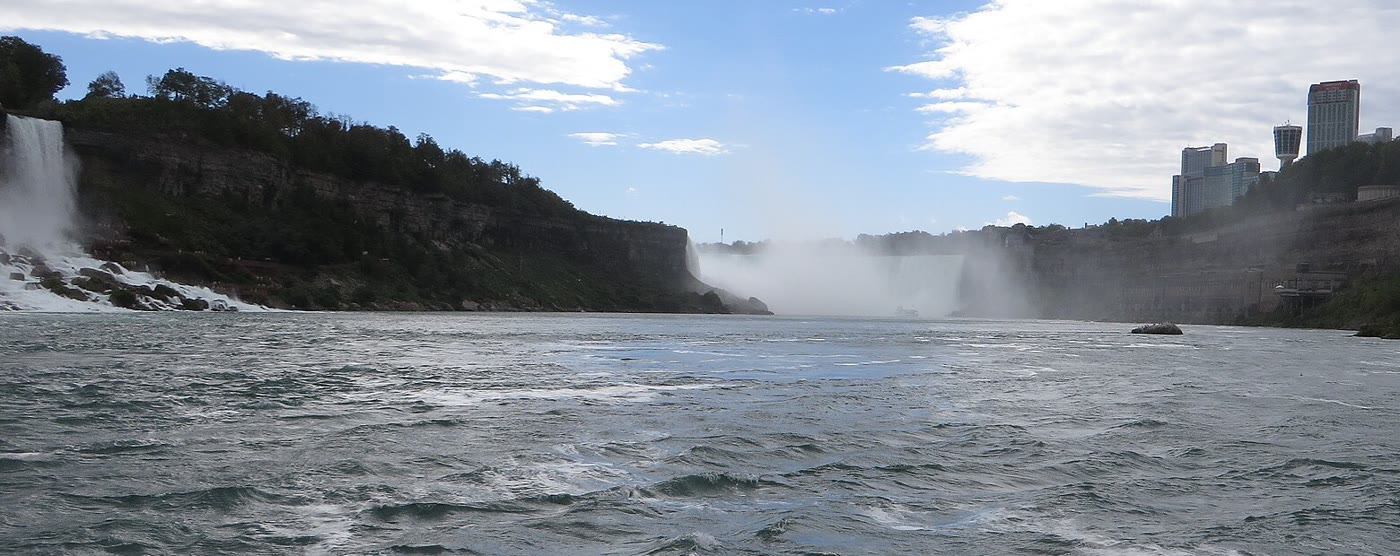
\includegraphics[width=\linewidth]{images/book5/b3-niagara-gorge.jpg}

{\scriptsize Ngarai Niagara, memandang ke hulu ke arah Horseshoe Falls dalam
kabutnya, American Falls di tepi kiri. Foto: Ken Lund,
CC BY-SA 2.0 (dipotong).}
\end{minipage}
\end{inthefield}
% ledger: ijc18:niagara, photo:b3-niagara-gorge


\section{Erosi glasial}\label{sec:b3:quantitative-geomorphology:glacial}

Gletser yang meluncur di atas dasarnya (gelincir basal,
Bab~\ref{ch:b3:glaciology}) mengikisnya melalui abrasi, ketika puing yang tertahan dalam
es menggerus batuan, dan melalui pencabutan, ketika gletser menarik keluar blok yang telah longgar
oleh retakan. Keduanya sebanding dengan kecepatan peluncuran.

\begin{definition}[Hukum erosi glasial]\label{def:b3:quantitative-geomorphology:glacial}
Yang disebut \emph{hukum erosi glasial}\index{hukum erosi glasial} memberikan laju
erosi dasar gletser sebagai $E = K_G\,u_s^{\,l}$, dengan $u_s$ adalah
kecepatan peluncuran, $K_G$ koefisien dan $l$ eksponen.
\end{definition}

Model bentang alam biasanya mengambil $l = 1$, dengan nilai antara 1 dan 2 yang juga digunakan.
Sebuah kompilasi 38 gletser, yang laju erosinya membentang lima orde
besaran, menemukan erosi berkorelasi dengan kecepatan peluncuran, dengan $l = 0.65$ dan
$K_G = 10^{-4}$ untuk $E$ dalam meter per tahun: erosi paling cepat terjadi di bawah gletser beriklim sedang
yang diberi salju melimpah, yang meluncur cepat. Karena es paling tebal
dan paling cepat sepanjang sumbu lembah, dasar lembah lebih diperdalam daripada
sisinya, dan lembah itu memperoleh bentuk U.
% ledger: cook20:glacial

\begin{definition}[Gergaji glasial]\label{def:b3:quantitative-geomorphology:buzzsaw}
Yang disebut \emph{gergaji glasial}\index{gergaji glasial} adalah batas yang ditetapkan pada
ketinggian pegunungan oleh gletser: di tempat batuan naik di atas ketinggian
tempat gletser terbentuk, gletser mengikisnya secepat batuan itu naik, berapa pun
laju pengangkatannya, sehingga puncak dan elevasi rata-rata berkumpul di dekat ketinggian itu.
\end{definition}

\section{Tektonika dan erosi}\label{sec:b3:quantitative-geomorphology:tectonics}

\begin{definition}[Keadaan tunak topografi]\label{def:b3:quantitative-geomorphology:steady-state}
Bentang alam berada dalam \emph{keadaan tunak topografi}\index{keadaan tunak topografi}
ketika laju erosinya sama dengan laju pengangkatan batuan di semua tempat, sehingga
elevasinya tidak berubah meskipun batuan melewatinya.
\end{definition}

Laju yang diukur dalam rentang waktu berbeda menguji keadaan tersebut. \omterm{def:b3:advanced-geochronology:cosmogenic}{Nuklida kosmogenik}
dalam pasir sungai memberikan laju erosi rata-rata suatu cekungan selama
waktu yang dibutuhkan untuk menghilangkan lapisan berorde panjang atenuasi
produksinya, sekitar \qty{55}{cm} batuan; \omterm{def:b3:orogenic-wedges:thermochronology}{termokronometer} dan \omterm{def:b3:orogenic-wedges:age-elevation}{hubungan umur--elevasinya} memberikan
laju ekshumasi selama jutaan tahun. Jika keduanya saling sepakat
dan sepakat dengan laju pengangkatan, bentang alam mungkin berada dalam \omterm{def:b3:quantitative-geomorphology:steady-profile}{keadaan tunak}; jika
laju jangka pendek di hilir lebih cepat daripada di hulu,
sebuah \omterm{def:b3:quantitative-geomorphology:knickpoint}{titik tekuk} sedang melintas. Pengambilan batuan juga meringankan
litosfer, yang kemudian naik sebagai responsnya.
% ledger: zech04:exposure

\begin{definition}[Pantulan isostatik erosional]\label{def:b3:quantitative-geomorphology:rebound}
Yang disebut \emph{pantulan isostatik erosional}\index{pantulan isostatik erosional} adalah
naiknya permukaan batuan suatu wilayah dalam kesetimbangan isostatik sebagai
respons terhadap massa yang dihilangkan oleh erosi.
\end{definition}

\begin{proposition}[Puncak naik seiring lembah makin dalam]\label{prop:b3:quantitative-geomorphology:rebound}
Dalam isostasi Airy dengan kerak bermassa jenis $\rho_c$ di atas mantel bermassa jenis
$\rho_m$, menghilangkan ketebalan rata-rata $\bar e$ dari kerak di suatu wilayah menaikkan
seluruh wilayah sebesar $(\rho_c/\rho_m)\,\bar e$. Jika erosi hanya terbatas
pada lembah, puncak yang tidak terkikis naik sebesar jumlah itu, sementara rata-rata
permukaan hanya turun sebesar $(1 - \rho_c/\rho_m)\,\bar e$.
\end{proposition}

\begin{proof}
Kompensasi menuntut agar massa setiap kolom di atas suatu kedalaman tetap
sama. Menghilangkan ketebalan $\bar e$ kerak, dirata-ratakan di atas luas
kompensasi, menurunkan massa per satuan luas sebesar $\rho_c \bar e$;
menggantinya menuntut mantel mengalir masuk pada kedalaman, sehingga mengangkat dasar
kolom, dan segala yang ada di atasnya, sebesar $\delta$ dengan $\rho_m \delta = \rho_c \bar
e$. Puncak yang tidak kehilangan batuan naik sebesar $\delta$; permukaan rata-rata kehilangan
$\bar e$ dan memperoleh $\delta$.
\end{proof}

Massa jenis kerak terbobot ketebalan pada model acuan Bumi adalah
\qty{2.72}{g/cm^3} dan massa jenis mantel di bawah Moho \qty{3.38}{g/cm^3},
dengan rasio 0.80: dari setiap seratus meter batuan yang terkikis, permukaan rata-rata
kehilangan hanya dua puluh. Penorehan yang dalam pada dataran tinggi tua dengan demikian dapat menaikkan
puncaknya meskipun dataran tinggi itu terus terkikis.
% ledger: prem:crust-mantle-ratio

\begin{omfigure}
\begin{tikzpicture}[x=0.6cm, y=0.6cm, font=\scriptsize]
\begin{scope}
\fill[omDef!12] (0,0) rectangle (8,4);
\draw[thick] (0,4) -- (8,4);
\draw[densely dashed] (0,0) -- (8,0);
\node[anchor=north] at (4,-0.1) {dasar kerak};
\node at (4,2) {kerak $\rho_c$};
\node at (4,-1.2) {mantel $\rho_m$};
\node[anchor=south] at (4,4.1) {sebelum};
\end{scope}
\begin{scope}[xshift=6.2cm]
\fill[omDef!12] (0,0.8) -- (0,4.8) -- (1.4,4.8) -- (2.0,2.4) -- (2.6,4.8) -- (5.4,4.8) -- (6.0,2.4) -- (6.6,4.8) -- (8,4.8) -- (8,0.8) -- cycle;
\draw[thick] (0,4.8) -- (1.4,4.8) -- (2.0,2.4) -- (2.6,4.8) -- (5.4,4.8) -- (6.0,2.4) -- (6.6,4.8) -- (8,4.8);
\draw[black!50, densely dashed] (0,4) -- (8,4);
\draw[densely dashed] (0,0.8) -- (8,0.8);
\draw[densely dashed, black!40] (0,0) -- (8,0);
\draw[<->, omThm] (8.3,4.05) -- (8.3,4.75) node[midway, right] {$\delta$};
\draw[<->, omThm] (8.3,0.05) -- (8.3,0.75) node[midway, right] {$\delta$};
\node[anchor=west, font=\scriptsize] at (8.1,2.4) {$\delta = (\rho_c/\rho_m)\,\bar e$};
\node[anchor=south] at (4,5.0) {setelah penorehan lembah};
\node[anchor=north] at (2.0,2.3) {lembah};
\end{scope}
\end{tikzpicture}

\par\smallskip{\small \omterm{def:b3:quantitative-geomorphology:rebound}{Pantulan isostatik erosional}, skematik. Penorehan
lembah menghilangkan ketebalan rata-rata $\bar e$ dari kerak; kolom naik sebesar
$\delta = (\rho_c/\rho_m)\bar e$ di dasarnya dan di puncaknya yang tidak tersentuh
(garis putus-putus abu-abu adalah permukaan lama).}\label{fig:b3:quantitative-geomorphology:rebound}
\end{omfigure}

\section{Latihan}

\begin{exercise}[$\star$]\label{exo:b3:quantitative-geomorphology:1}
Sebuah tebing pantai dengan pergeseran \qty{4}{m} ($a = \qty{2}{m}$) berada pada
lereng medan jauh sebesar 0.04, dan gradien tercuramnya kini 0.30. Hitung
$\kappa t$, lalu umur tebing itu dengan $\kappa = \qty{5e-3}{m^2/yr}$.
\end{exercise}
% ledger: whipple04:scarp-erf, whipple04:scarp-kappa

\begin{exercise}[$\star$]\label{exo:b3:quantitative-geomorphology:2}
Survei lidar memberikan kelengkungan puncak bukit sebesar \qty{-0.012}{m^{-1}} pada punggungan
dengan difusivitas \qty{4e-3}{m^2/yr}. Hitung laju erosinya dalam
\unit{mm/yr}, dan relief antara puncaknya dan alur
berjarak \qty{80}{m}, dengan asumsi \omterm{def:b3:quantitative-geomorphology:steady-profile}{keadaan tunak}.
\end{exercise}

\begin{exercise}[$\star$]\label{exo:b3:quantitative-geomorphology:3}
Dengan $m = 0.5$, $n = 1$ dan $K = \qty{2e-6}{yr^{-1}}$, hitung
laju penorehan sungai dengan daerah tangkapan \qty{25}{km^2} pada gradien 0.01.
Apa satuan $K$ untuk $m$ dan $n$ yang umum?
\end{exercise}

\begin{exercise}[$\star$]\label{exo:b3:quantitative-geomorphology:4}
Tiga sungai menunjukkan \omterm{def:b3:quantitative-geomorphology:knickpoint}{titik tekuk}: (a) tempat lapisan batu pasir memotong lembah
yang tergerus pada serpih; (b) tempat sungai memotong sesar normal aktif dari
dinding bawah ke dinding gantung; (c) pada setiap sungai di suatu cekungan, semuanya pada kira-kira
ketinggian yang sama, beberapa kilometer di atas pesisir yang naik saat
gempa bumi. Mana yang tetap dan mana yang akan bermigrasi?
\end{exercise}

\begin{exercise}[$\star\star$]\label{exo:b3:quantitative-geomorphology:5}
Untuk $m = 1$ dan $n = 2$, hitung $\theta$ dan gradien \omterm{def:b3:quantitative-geomorphology:steady-profile}{keadaan tunak} di tempat $A =
\qty{10}{km^2}$, dengan $U = \qty{0.1}{mm/yr}$ dan $K = 10^{-9}$ dalam meter dan
tahun.
Dengan faktor berapa kecuraman berubah jika $U$ dua kali lipat? Bandingkan dengan $n =
1$.
\end{exercise}

\begin{exercise}[$\star\star$]\label{exo:b3:quantitative-geomorphology:6}
Daerah tangkapan sungai bertambah seiring jarak $d$ dari pemisah airnya sebagai $A =
c\,d^{h}$. Tunjukkan bahwa, diukur ke hulu dari muaranya pada $d = L$,
\[
\chi(d) = \frac{A_0^{\theta}}{c^{\theta}}\,\frac{L^{p} - d^{p}}{p},
\qquad p = 1 - h\theta ,
\]
dan hitung untuk $c = 2$ (SI), $h = 1.8$, $\theta = 0.45$, $A_0 =
\qty{1}{km^2}$, $L = \qty{20}{km}$, dan $d = \qty{5}{km}$.
\end{exercise}

\begin{exercise}[$\star\star$]\label{exo:b3:quantitative-geomorphology:7}
Dengan $n = 1$, $m = 0.5$ dan $K = \qty{2e-6}{yr^{-1}}$, hitung
kecepatan rambat \omterm{def:b3:quantitative-geomorphology:knickpoint}{titik tekuk} tempat $A = \qty{100}{km^2}$, dalam m/ka, dan
waktu yang dibutuhkan untuk menempuh \qty{5}{km} pada kecepatan itu. Mengapa
sebenarnya butuh waktu lebih lama?
\end{exercise}

\begin{exercise}[$\star\star$]\label{exo:b3:quantitative-geomorphology:8}
Lembah sedalam \qty{600}{m}, yang rata-rata menempati \qty{40}{\percent} dari
luas suatu dataran tinggi, tergerus ke dalamnya. Dengan $\rho_c/\rho_m = 0.80$, hitung
ketebalan rata-rata yang tererosi, naiknya puncak, dan perubahan
ketinggian rata-rata.
\end{exercise}
% ledger: prem:crust-mantle-ratio

\begin{exercise}[$\star\star$]\label{exo:b3:quantitative-geomorphology:9}
Sebuah \omterm{def:b3:quantitative-geomorphology:soil-production}{fungsi produksi tanah} memiliki $P_0 = \qty{0.3}{mm/yr}$ dan $h_0 =
\qty{0.5}{m}$. Hitung ketebalan tanah \omterm{def:b3:quantitative-geomorphology:steady-profile}{keadaan tunak} untuk erosi pada
\qty{0.05}{mm/yr} dan pada \qty{0.2}{mm/yr}. Apa yang terjadi pada
\qty{0.4}{mm/yr}?
\end{exercise}

\begin{exercise}[$\star\star\star$]\label{exo:b3:quantitative-geomorphology:10}
Sebuah bukit dalam \omterm{def:b3:quantitative-geomorphology:steady-profile}{keadaan tunak} tererosi dengan laju $E = \qty{0.1}{mm/yr}$ dan $\kappa =
\qty{5e-3}{m^2/yr}$ dan hukum nonlinier gradien kritis, dengan mengambil
$S_c = 1.2$ untuk soal ini. Tunjukkan bahwa fluks pada jarak $x$ dari
pemisah adalah $E x$, selesaikan untuk gradiennya, dan hitung pada 20, 50, 100, dan
\qty{200}{m}. Bandingkan dengan difusi linier dan deskripsikan bentuk
bukit.
\end{exercise}

\begin{exercise}[$\star\star\star$]\label{exo:b3:quantitative-geomorphology:11}
Tunjukkan bahwa waktu respons jaringan sungai terhadap perubahan di muaranya,
untuk $n = 1$, adalah $\chi_h/(K A_0^m)$, dengan $\chi_h$ adalah nilai terbesar dari
$\chi$ pada kepala alur. Hitung untuk sungai dataran tinggi pada gambar-gambar
($A_0 = \qty{1}{km^2}$, $m = 0.5$, $K = \qty{e-6}{yr^{-1}}$), pertama untuk
batang utama saja, yang kepalanya berada pada $\chi = \qty{5464}{m}$, lalu untuk jaringan,
yang kepala tertingginya, pada anak sungai 1, berada pada $\chi = \qty{7237}{m}$.
\end{exercise}

\begin{exercise}[$\star\star\star$]\label{exo:b3:quantitative-geomorphology:12}
Dalam jaringan dengan $n = 1$ dan $U$ seragam, satu anak sungai mengalir di atas batuan dua kali
lebih mudah tererosi daripada sisanya ($2K$) di atas pertemuannya, pada $\chi_j$. Tunjukkan bahwa
garis \omterm{def:b3:quantitative-geomorphology:steady-profile}{keadaan tunaknya} pada bidang $(\chi, z)$ memiliki setengah kemiringan dari
batang utama di atas $\chi_j$, dan bahwa \omterm{def:b3:quantitative-geomorphology:knickpoint}{titik tekuk} yang lahir di muara mencapai,
pada saat \omterm{def:b3:quantitative-geomorphology:knickpoint}{titik tekuk} batang utama berada di $\chi_k > \chi_j$, titik
dengan $\chi = \chi_j + 2(\chi_k - \chi_j)$ pada anak sungai tersebut.
\end{exercise}

\section{Soal: Air terjun Sungai Varden}

\begin{problem}[{Soal akhir pekan --- profil, kecuraman, dan erodibilitas
sungai dataran tinggi rekaan, dan umur air terjunnya}]
\label{pb:b3:quantitative-geomorphology:1}
Di sebelah barat Perbukitan Varden, sungai mengalirkan dataran tinggi sekis sebelum
memasuki peta di tepi barat, pada ketinggian \qty{170}{m}. Di hulu
titik itu, yakni muaranya, batang utama panjangnya \qty{12}{km} dari pemisahnya,
dengan daerah tangkapan $A = 4.5\,d^{1.7}$ (\unit{m^2}, $d$ dalam meter dari
pemisah) dan kepala alur pada $d = \qty{300}{m}$. Ambil laju pengangkatan batuan
sama dengan laju denudasi cekungan Sungai Varden yang diperoleh dari muatannya dalam volume Tahun 1,
\qty{43}{m/Ma}. Ambil $n = 1$ dan luas acuan $A_0 = \qty{1}{km^2}$.
Sebuah air terjun setinggi \qty{25}{m} berada pada batang utama \qty{4.60}{km} di hulu
muara. Semua nilai adalah rekaan.

\medskip\noindent\textbf{Bagian I --- Profil.}
\begin{enumerate}
\item Hitung luas daerah tangkapan di muara dan di kepala alur.
\item Gradien yang diukur pada ruas sepanjang \qty{200}{m}, menjauhi
  air terjun:

  \smallskip
  {\small\begin{tabular}{l*{6}{c}}
  $A$ (\unit{km^2}) & 0.388 & 0.587 & 0.888 & 1.345 & 2.036 & 3.082 \\
  $S$ & 0.06641 & 0.05026 & 0.04888 & 0.03322 & 0.03688 & 0.02688 \\[2pt]
  $A$ (\unit{km^2}) & 4.665 & 7.061 & 10.69 & 16.18 & 24.49 & 37.08 \\
  $S$ & 0.01921 & 0.01713 & 0.01545 & 0.01419 & 0.007922 & 0.007855
  \end{tabular}}

  \smallskip
  Taksir \omterm{def:b3:quantitative-geomorphology:indices}{indeks kecekungan} dari titik pertama dan titik terakhir.
\item Kemiringan kuadrat terkecil dari $\log S$ terhadap $\log A$ adalah $-0.466$.
  Apakah itu konsisten dengan $\theta = 0.5$?
\item Dengan $\theta_{\mathrm{ref}} = 0.5$, hitung $k_{sn} = S A^{0.5}$ ($A$ dalam
  \unit{m^2}) untuk titik pertama dan titik terakhir, serta jelaskan apa
  yang diwakili oleh rata-rata geometris dari dua belas nilai, \qty{45.1}{m}.
\item Mengapa gradien jauh lebih menyebar daripada ketinggian?
\item Dengan menggunakan rumus latihan chi, hitung $\chi$ pada $d =
  \qty{9.00}{km}$, titik di bawah air terjun.
\end{enumerate}

\medskip\noindent\textbf{Bagian II --- Kecuraman dan erodibilitas.}
\begin{enumerate}[resume]
\item Sungai berada pada \qty{193.4}{m} di $d = \qty{9.00}{km}$. Hitung
  kemiringan plot chi di bawah air terjun dan kecuraman $k_{sn}$.
\item Di antara taksiran $k_{sn}$ ini dan taksiran luas-kemiringan, mana yang
  akan kamu percayai, dan mengapa?
\item Dengan asumsi \omterm{def:b3:quantitative-geomorphology:steady-profile}{keadaan tunak} di bawah air terjun, hitung $K$ dari
  laju pengangkatan.
\item Periksa bahwa laju penggerusan di muara, yang gradiennya
  0.00691, sama dengan laju pengangkatan.
\item Hitung kecepatan rambat \omterm{def:b3:quantitative-geomorphology:knickpoint}{titik tekuk} di muara dan di
  air terjun, dalam m/ka.
\item Hitung elevasi kepala alur pada profil \omterm{def:b3:quantitative-geomorphology:steady-profile}{keadaan tunak}, serta
  relief batang utama.
\end{enumerate}

\medskip\noindent\textbf{Bagian III --- Air terjun.}
\begin{enumerate}[resume]
\item Mengapa, dengan $n = 1$, air terjun mempertahankan tinggi
  sama dengan penurunan \omterm{def:b3:quantitative-geomorphology:knickpoint}{dasar erosi}?
\item Hitung $\chi$ di air terjun.
\item Hitung waktu yang dibutuhkan \omterm{def:b3:quantitative-geomorphology:knickpoint}{titik tekuk} dari muara hingga
  posisinya sekarang.
\item Di mana \omterm{def:b3:quantitative-geomorphology:knickpoint}{titik tekuk} itu akan berada \qty{300}{ka} dari sekarang?
\item Anak sungai 3 bergabung dengan batang utama \qty{2.5}{km} di hulu muara; ia
  panjangnya \qty{5}{km}, dengan $A = 1.5\,s^{1.7}$ ($s$ dari pemisahnya sendiri).
  Di mana air terjunnya seharusnya berada?
\item Anak sungai 1 dan 2 bergabung dengan batang utama masing-masing 8 dan \qty{5}{km} di hulu
  muara. Jelaskan mengapa keduanya tidak memiliki air terjun.
\end{enumerate}

\medskip\noindent\textbf{Bagian IV --- Lereng dan umur.}
\begin{enumerate}[resume]
\item Survei lidar di atas air terjun memberikan kelengkungan puncak bukit sebesar
  \qty{-0.0086}{m^{-1}}. Dengan $\kappa = \qty{5e-3}{m^2/yr}$, hitung
  laju erosi dan bandingkan dengan laju pengangkatan.
\item Lereng-lereng bukit itu panjangnya sekitar \qty{150}{m}. Bandingkan waktu respons
  mereka $L^2/\kappa$ dengan umur yang diperoleh pada Bagian III.
\item Deskripsikan lereng bukit di bawah air terjun saat ini, serta bagaimana
  mereka akan berubah.
\item Laju pengangkatan diketahui dengan ketelitian \qty{20}{\percent}. Berikan rentang
  umurnya.
\item Bagaimana air terjun akan berkembang jika $n$ bernilai 2?
\item Berikan umur penurunan \omterm{def:b3:quantitative-geomorphology:knickpoint}{dasar erosi}.
\end{enumerate}
\end{problem}
% ledger: whipple04:steepness, whipple04:scarp-kappa
